\ifdefined\included
\else
\documentclass[english,a4paper,11pt,twoside]{StyleThese}
\usepackage{amsmath,amssymb}             % AMS Math
\usepackage[T1]{fontenc}
\usepackage[utf8x]{inputenc}
\usepackage{babel}
\usepackage{datetime}

\usepackage{lmodern}
\usepackage{tabularx}
%\usepackage{tabular}
\usepackage{multirow}

\usepackage{subfigure}
\usepackage{fancyvrb}


\usepackage{hhline}
\usepackage[left=1.5in,right=1.3in,top=1.1in,bottom=1.1in,includefoot,includehead,headheight=13.6pt]{geometry}
\renewcommand{\baselinestretch}{1.05}

% Table of contents for each chapter

\usepackage[nottoc, notlof, notlot]{tocbibind}
\usepackage{minitoc}
\setcounter{minitocdepth}{2}
\mtcindent=15pt
% Use \minitoc where to put a table of contents

\usepackage{aecompl}


% Glossary / list of abbreviations

\usepackage[intoc]{nomencl}
\iftoggle{ThesisInEnglish}{%
\renewcommand{\nomname}{Glossary}
}{ %
\renewcommand{\nomname}{Liste des Abréviations}
}

\makenomenclature

% My pdf code

\usepackage{ifpdf}

\ifpdf
  \usepackage[pdftex]{graphicx}
  \DeclareGraphicsExtensions{.jpg}
  \usepackage[a4paper,pagebackref,hyperindex=true]{hyperref}
  \usepackage{tikz}
  \usetikzlibrary{arrows,shapes,calc}
\else
  \usepackage{graphicx}
  \DeclareGraphicsExtensions{.ps,.eps}
  \usepackage[a4paper,dvipdfm,pagebackref,hyperindex=true]{hyperref}
\fi

\graphicspath{{.}{images/}}

%% nicer backref links. NOTE: The flag ThesisInEnglish is used to define the
% language in the back references. Read more about it in These.tex

\iftoggle{ThesisInEnglish}{%
\renewcommand*{\backref}[1]{}
\renewcommand*{\backrefalt}[4]{%
\ifcase #1 %
(Not cited.)%
\or
(Cited in page~#2.)%
\else
(Cited in pages~#2.)%
\fi}
\renewcommand*{\backrefsep}{, }
\renewcommand*{\backreftwosep}{ and~}
\renewcommand*{\backreflastsep}{ and~}
}{%
\renewcommand*{\backref}[1]{}
\renewcommand*{\backrefalt}[4]{%
\ifcase #1 %
(Non cité.)%
\or
(Cité en page~#2.)%
\else
(Cité en pages~#2.)%
\fi}
\renewcommand*{\backrefsep}{, }
\renewcommand*{\backreftwosep}{ et~}
\renewcommand*{\backreflastsep}{ et~}
}

% Links in pdf
\usepackage{color}
\definecolor{linkcol}{rgb}{0,0,0.4} 
\definecolor{citecol}{rgb}{0.5,0,0} 
\definecolor{linkcol}{rgb}{0,0,0} 
\definecolor{citecol}{rgb}{0,0,0}
% Change this to change the informations included in the pdf file

\hypersetup
{
bookmarksopen=true,
pdftitle="Joint Action for Human-Robot Interaction",
pdfauthor="Sandra DEVIN", %auteur du document
pdfsubject="Thesis", %sujet du document
%pdftoolbar=false, %barre d'outils non visible
pdfmenubar=true, %barre de menu visible
pdfhighlight=/O, %effet d'un clic sur un lien hypertexte
colorlinks=true, %couleurs sur les liens hypertextes
pdfpagemode=None, %aucun mode de page
pdfpagelayout=SinglePage, %ouverture en simple page
pdffitwindow=true, %pages ouvertes entierement dans toute la fenetre
linkcolor=linkcol, %couleur des liens hypertextes internes
citecolor=citecol, %couleur des liens pour les citations
urlcolor=linkcol %couleur des liens pour les url
}

% definitions.
% -------------------

\setcounter{secnumdepth}{3}
\setcounter{tocdepth}{2}

% Some useful commands and shortcut for maths:  partial derivative and stuff

\newcommand{\pd}[2]{\frac{\partial #1}{\partial #2}}
\def\abs{\operatorname{abs}}
\def\argmax{\operatornamewithlimits{arg\,max}}
\def\argmin{\operatornamewithlimits{arg\,min}}
\def\diag{\operatorname{Diag}}
\newcommand{\eqRef}[1]{(\ref{#1})}

\usepackage{rotating}                    % Sideways of figures & tables
%\usepackage{bibunits}
%\usepackage[sectionbib]{chapterbib}          % Cross-reference package (Natural BiB)
%\usepackage{natbib}                  % Put References at the end of each chapter
                                         % Do not put 'sectionbib' option here.
                                         % Sectionbib option in 'natbib' will do.
\usepackage{fancyhdr}                    % Fancy Header and Footer

% \usepackage{txfonts}                     % Public Times New Roman text & math font
  
%%% Fancy Header %%%%%%%%%%%%%%%%%%%%%%%%%%%%%%%%%%%%%%%%%%%%%%%%%%%%%%%%%%%%%%%%%%
% Fancy Header Style Options

\pagestyle{fancy}                       % Sets fancy header and footer
\fancyfoot{}                            % Delete current footer settings

%\renewcommand{\chaptermark}[1]{         % Lower Case Chapter marker style
%  \markboth{\chaptername\ \thechapter.\ #1}}{}} %

%\renewcommand{\sectionmark}[1]{         % Lower case Section marker style
%  \markright{\thesection.\ #1}}         %

\fancyhead[LE,RO]{\bfseries\thepage}    % Page number (boldface) in left on even
% pages and right on odd pages
\fancyhead[RE]{\bfseries\nouppercase{\leftmark}}      % Chapter in the right on even pages
\fancyhead[LO]{\bfseries\nouppercase{\rightmark}}     % Section in the left on odd pages

\let\headruleORIG\headrule
\renewcommand{\headrule}{\color{black} \headruleORIG}
\renewcommand{\headrulewidth}{1.0pt}
\usepackage{colortbl}
\arrayrulecolor{black}

\fancypagestyle{plain}{
  \fancyhead{}
  \fancyfoot{}
  \renewcommand{\headrulewidth}{0pt}
}

%\usepackage{MyAlgorithm}
%\usepackage[noend]{MyAlgorithmic}
\usepackage[ED=MITT - STICIA, Ets=INP]{tlsflyleaf}
%%% Clear Header %%%%%%%%%%%%%%%%%%%%%%%%%%%%%%%%%%%%%%%%%%%%%%%%%%%%%%%%%%%%%%%%%%
% Clear Header Style on the Last Empty Odd pages
\makeatletter

\def\cleardoublepage{\clearpage\if@twoside \ifodd\c@page\else%
  \hbox{}%
  \thispagestyle{empty}%              % Empty header styles
  \newpage%
  \if@twocolumn\hbox{}\newpage\fi\fi\fi}

\makeatother
 
%%%%%%%%%%%%%%%%%%%%%%%%%%%%%%%%%%%%%%%%%%%%%%%%%%%%%%%%%%%%%%%%%%%%%%%%%%%%%%% 
% Prints your review date and 'Draft Version' (From Josullvn, CS, CMU)
\newcommand{\reviewtimetoday}[2]{\special{!userdict begin
    /bop-hook{gsave 20 710 translate 45 rotate 0.8 setgray
      /Times-Roman findfont 12 scalefont setfont 0 0   moveto (#1) show
      0 -12 moveto (#2) show grestore}def end}}
% You can turn on or off this option.
% \reviewtimetoday{\today}{Draft Version}
%%%%%%%%%%%%%%%%%%%%%%%%%%%%%%%%%%%%%%%%%%%%%%%%%%%%%%%%%%%%%%%%%%%%%%%%%%%%%%% 

\newenvironment{maxime}[1]
{
\vspace*{0cm}
\hfill
\begin{minipage}{0.5\textwidth}%
%\rule[0.5ex]{\textwidth}{0.1mm}\\%
\hrulefill $\:$ {\bf #1}\\
%\vspace*{-0.25cm}
\it 
}%
{%

\hrulefill
\vspace*{0.5cm}%
\end{minipage}
}

\let\minitocORIG\minitoc
\renewcommand{\minitoc}{\minitocORIG \vspace{1.5em}}

\usepackage{multirow}
%\usepackage{slashbox}

\newenvironment{bulletList}%
{ \begin{list}%
	{$\bullet$}%
	{\setlength{\labelwidth}{25pt}%
	 \setlength{\leftmargin}{30pt}%
	 \setlength{\itemsep}{\parsep}}}%
{ \end{list} }

\newtheorem{definition}{Définition}
\renewcommand{\epsilon}{\varepsilon}

% centered page environment

\newenvironment{vcenterpage}
{\newpage\vspace*{\fill}\thispagestyle{empty}\renewcommand{\headrulewidth}{0pt}}
{\vspace*{\fill}}

\usepackage{tablefootnote}

\sloppy
\begin{document}
\setcounter{chapter}{0} %% Numéro du chapitre précédent ;)
\dominitoc
\faketableofcontents
\fi

\chapter{From Human-Human Joint Action to Human-Robot Joint Action}
\minitoc

\section{Joint Action Theory}

A first step to endow robots with the ability to perform Joint Actions with humans is to understand how humans act together. As a working definition of Joint Action, we will use the one from \cite{sebanz2006joint}:

\begin{quote}
\textit{Joint action can be regarded as any form of social interaction whereby two or more individuals coordinate their actions in space and time to bring about a change in the environment.}
\end{quote}

A given number of prerequisites are needed for these individuals to achieve the so-called Joint Action. First of all, they need to agree on the change they want to bring in the environment, the conditions under which they will stay engaged in its realization and the way to do it. A number of works have studied this problematic, named \textit{commitment}, which I will develop in Sec.~\ref{subsec:commitment}. Then, as mentioned in the definition, the individuals need to coordinate their actions in space and time. This will be studied in Sec.~\ref{subsec:coordination}. Finally, in order to coordinate, each individual needs to be aware of the other, he needs to be able to perceive him and predict his actions. This part will be develop in Sec.~\ref{subsec:prediction}.
\accom{qu'est ce que tu veux dire qd tu dis, `` a number of works have studied this problematic, named commitment'' car avant tu parles de : 1) they need to agree on the change they want to bring in the environment, 2) the conditions under which they will stay engaged in its realization, 3) the conditions under which they will do it (ie the way to do it). Est ce que tu veux dire que tout çà cela recouvre la notion de commitment ? çà me semble pas correcte}

\subsection{Commitment}

\label{subsec:commitment}

The first prerequisite to achieve a Joint Action is to have a \textit{goal} to pursue and the \textit{intention} to achieve it. Let's define what is called a \textit{goal} and an \textit{intention} for a single person before going to a \textit{joint goal} and a \textit{joint intention}.

In \cite{tomasello2005understanding}, Tomasello et al. define what they call a \textit{goal} and an \textit{intention} and illustrate these definitions with an example and an associated figure (fig.~\ref{fig:intention}) where a person wants to open a box.

\begin{figure}[!h]
	\centering
    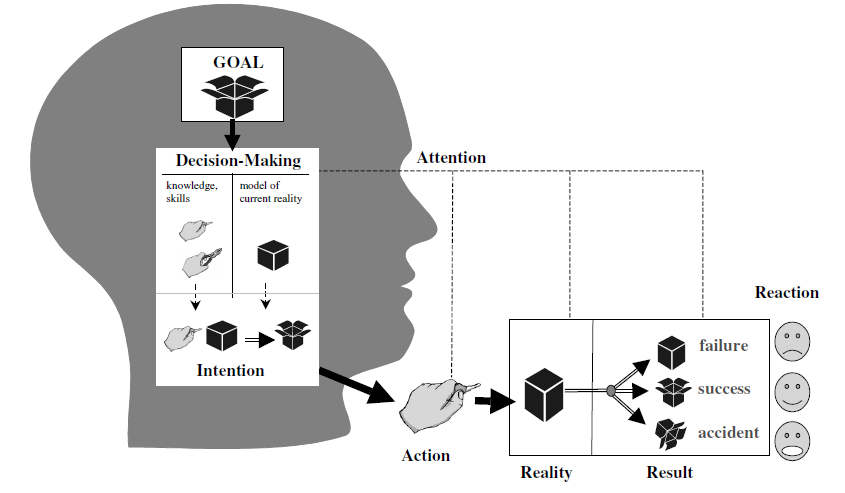
\includegraphics[width=0.8\textwidth]{figs/Chapter1/intention.png}
    \caption{Illustrative example of an intentional action by Tomasello et al. Here the human has for \textit{goal} to open the box. He chooses a means to perform it and so forms an \textit{intention}.}
    \label{fig:intention}
\end{figure}
\accom{es tu sûr de la définition du but ? est ce que le but c'est d'ouvrir la boite ou d'avoir une boite ouverte à la fin ? il me semble que ce n'est pas équivalent, non ?}
A \textit{goal} is defined here as the representation of the desired state by the agent (in the example, the goal is an open box) and, based on Bratman's work \cite{bratman1989intention}, an \textit{intention} is defined as an action plan the agent commits to in pursuit of a goal (in the example, the intention is to use a key to open the box). The \textit{intention} includes both a \textit{goal} and the means to achieve it. 
\accom{alors l'intention c'est le goal et le plan ? ou ce n'est pas ce que tu veux dire ?}

In a same way, Cohen and Levesque propose in \cite{cohen1991teamwork} a formal definition of what they call a \textit{persistent goal}:

\begin{quote}
\textbf{Definition: } An agent has a \textit{persistent goal} relative to \textit{q} to achieve \textit{p} iff:
\begin{enumerate}
\item she believes that \textit{p} is currently false;
\item she wants \textit{p} to be true eventually;
\item it is true (and she knows it) that (2) will continue to hold until she comes to believe either that \textit{p} is true, or that it will neither be true, or that \textit{q} is false.
\end{enumerate}
\end{quote}

However, their definition of an \textit{intention} differs a little from the previous one. They define an \textit{intention} as a commitment to act in a certain mental state:

\begin{quote}
\textbf{Definition:} An agent \textit{intends} relative to some conditions to do an action just in case she has a persistent goal (relative to that condition) of having done the action, and, moreover, having done it, believing throughout that she is doing it.
\end{quote}

The \textit{intention} still includes the \textit{goal} but here it concerns more the fact that the agent commits to achieving the goal than the way to achieve it.

Let's now apply these principles to a Joint Action. One of the best known definition of \textit{joint intention} is the one of Bratman \cite{bratman1993shared}:
\accom{il faudrait vérifier qu'il n'a pas changé un peu de définition depuis... notamment voir si il y a une différence entre shared et joint intention ? notamment dans son bouquin shared agency, dans le papier qu'on avait fait avec elle Elisabeth avait fait un laius sur çà, il faudrait que je te retrouve çà si çà te dit. Ca peut valoir le coup de regarder çà : https://jeannicod.ccsd.cnrs.fr/file/index/docid/872152/filename/Pacherie-joint_agency-Synthese-2013.pdf et aussi ce qu'a fait Butterfill}}

\begin{quote}
We intend to \textit{J} if and only if:
\begin{enumerate}
\item (a) I intend that we \textit{J} and (b) you intend that we \textit{J}.
\item I intend that we \textit{J} in accordance with and because of 1\textit{a}, 1\textit{b}, and meshing subplans of 1\textit{a} and 1\textit{b}; you intend that we \textit{J} in accordance with and because of 1\textit{a}, 1\textit{b}, and meshing subplans of 1\textit{a} and 1\textit{b}.
\item 1 and 2 are common knowledge between us.
\end{enumerate}
\end{quote}

This definition is taken back and illustrated by Tomasello et al. in \cite{tomasello2005understanding} where they reuse the example of the box to open (fig~\ref{fig:intention_jointe}).

\begin{figure}[!h]
	\centering
    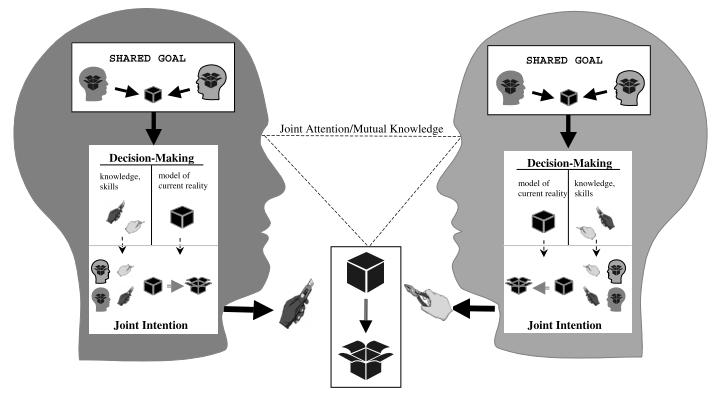
\includegraphics[width=0.75\textwidth]{figs/Chapter1/intention_jointe.png}
    \caption{Illustrative example of a collaborative activity by Tomasello et al. Here the humans have for \textit{shared goal} to open the box together. They choose a means to perform it which takes into account the other capabilities and so form a \textit{joint intention}.}
    \label{fig:intention_jointe}
\end{figure}

The \textit{shared goal} is defined as the representation of a desired state plus the fact that it will be done in collaboration with other person(s) (in the example, they will open the box together) and a \textit{joint intention} is defined as a collaborative plan the agents commit to in order to achieve the \textit{shared goal} and which takes into account both agents individual plans (here an agent will hold the box with the clamp while the other open it with the cutter).

In a same way, Cohen and Levesque extend their definition of \textit{persistent goal} and \textit{intention} to a collaborative activity. They first define a \textit{weak achievement goal} as:
\begin{quote}
\textbf{Definition: } An agent has a \textit{weak achievement goal} relative to \textit{q} and with respect to a team to bring about \textit{p} if either of these conditions holds:
\begin{itemize}
\item The agent has a normal achievement goal to bring about \textit{p}, that is, the agent does not yet believe that \textit{p} is true and has \textit{p} eventually being true as goal.
\item The agent believes that \textit{p} is true, will never be true, or is irrelevant (that is, \textit{q} is false), \textit{but} has as a goal that the status of \textit{p} be mutually believed by all the team members.
\end{itemize}
\end{quote}

They then use this definition to define a \textit{joint persistent goal}:
\begin{quote}
\textbf{Definition: } A team of agents have a \textit{joint persistent goal} relative to \textit{q} to achieve \textit{p} just in case
\begin{itemize}
\item they mutually believe that \textit{p} is currently false;
\item they mutually know they all want \textit{p} to eventually be true;
\item it is true (and mutual knowledge) that until they come to mutually believe that \textit{p is true}, that \textit{p} will never be true, or that \textit{q} is false, they will continue to mutually believe that they each have \textit{p} as a weak achievement goal relative to \textit{q} and with respect to the team.
\end{itemize}
\end{quote}

They finally define a \textit{joint intention} as:
\begin{quote}
\textbf{Definition:} A team of agents \textit{jointly intends}, relative to some escape condition, to do an action iff the members have a joint persistent goal relative of that condition of their having done the action and, moreover, having done it mutually believing throughout that they were doing it.
\end{quote}

As previously, the definitions of Cohen and Levesque do no take into account the way to achieve the \textit{shared goal}, however, they introduce the interesting idea that agents are also engaged to communicate about the state of the \textit{shared goal}.

Concerning the way to achieve a \textit{shared goal}, mentioned into the definition of the \textit{joint intention} of Tomasello et al., Grosz and Sidner initially introduce and formalize the notion of \textit{Shared Plan} in \cite{grosz1988plans}, which is extended in \cite{grosz1999evolution}. The key properties of their model are as follows:
\begin{quote}
\begin{enumerate}
\item it uses individual intentions to establish commitment of collaborators to their joint activity
\item it establishes an agent's commitments to its collaborating partners' abilities to carry out their
individual actions that contribute to the joint activity
\item it accounts for helpful behavior in the context of collaborative activity
\item it covers contracting actions and distinguishes contracting from collaboration
\item the need for agents to communicate is derivative, not stipulated, and follows from the general
commitment to the group activity
\item the meshing of subplans is ensured it is also derivative from more general constraints.
\end{enumerate}
\end{quote}

With their definition, each agent does not necessarily know the whole \textit{Shared Plan} but only his own individual plan and the meshing subparts of the plan. The group has a \textit{Shared Plan}, but no individual member necessarily has the whole \textit{Shared Plan}.

In conclusion, the concepts concerning the commitment of agents to a collaborative activity that we will use in this thesis can be summarized as:
\begin{itemize}
\item A \textit{goal} will be represented as a desired state.
\item A\textit{shared goal} will be considered as a \textit{goal} to be achieved in collaboration with other partner(s). An agent is considered engaged in a \textit{shared goal} if he believes the goal is currently false, he wants the goal to be true and he will not give up on the goal unless he knows that the goal is achieved, not feasible or not relevant any more and he knows that his partners are aware of it.
\item A \textit{joint intention} will include a \textit{shared goal} and the way to realize it, represented as a \textit{Shared Plan} which will take into account the capacities of each agent and the potential conflicts between their actions. This \textit{Shared Plan} will not be necessarily completely known by all members of the group but all individuals will know their part of the plan and the meshing subparts.
\end{itemize}

\accom{çà pourrait valoir le coup de prendre un exemple fil rouge pour lesquels tu donnerais les implications de ces choix non ? e.g. si ton but est un état voulu alors il se définit de tel façon dans l'exemple etc.. ?}
\accom{dans tous les cas, çà vaudrait peut etre le coup de faire relire çà à Elisabeth, qu'en dis tu ?}

\subsection{Perception and prediction}

\label{subsec:prediction}

One important thing for an agent when performing a Joint Action is to be able to perceive and predict the actions of his partner and their effects. Based on the works in \cite{sebanz2006joint}, \cite{pacherie2011phenomenology} and \cite{obhi2011moving} we identified several necessary abilities for this predictions:

\paragraph{Joint attention:} The capacity for an agent to share focus with his partner allows to share a representation of objects and events. It brings a better understanding of the other agent's knowledge and where his attention is focused and so, it helps the prediction of his possible next actions. Moreover, there should be a mutual manifestation of this joint attention, meaning that we should show that we share the other attention. 

\paragraph{Action observation:} Several studies have shown that when someone observes another person executing an action, a corresponding representation of the action is formed for the observer \cite{rizzolatti2004mirror}. This is done by what has been called the \textit{mirror-neuron} system. This behavior allows the observer to predict the outcomes of the actor's action. 

\paragraph{Co-representation:} An agent needs to have a representation of his partner, including his goal, his capacities and the social rules he is following. Indeed, having this representation will help to predict his future actions. For example, a pedestrian who sees a red traffic light will be able to predict that the car drivers will stop. In a same way, if you know that someone is aiming to go out shopping, you will be able to predict that he will look for the key of the car.

\accom{j'ai l'impression que tu mélanges Action observation et Co-representation ? (moi j'avais plutot retenue Intentional action understanding d'une part et Shared Task representation d'autre part, mais), ce que je veux dire c'est que est ce que Action observation est une ability ? (puisque c'est de çà que tu parles ici) et dans la définition que tu donnes c'est plutôt le fait qu'on a ou qu'on représente ces actions non ? ensuite qd tu parles de co-representation tu parles bien d'avoir une représentation de l'autre et de ce qu'il peut/veut faire mais tu ne parles pas de representation partagée de plan ou de tâches, c'est complémentaire à mon sens mais ne faut-il pas le citer ? }

\paragraph{Agency:} Sometimes, when there is a close link between an action performed by oneself and an action performed by someone else, it can be hard to distinguish who caused a particular effect. The capacity to attribute the effects to the right actor is called the sense of \textit{Agency}. This sense of \textit{Agency} is important in Joint Action in order to correctly predict the effects of each action.
\accom{j'avais mis çà derrière self-other distinction mais j'aime bien l'idée de considérer çà comme dépendant de l'Agency}

\bigskip
Based on the same works as before and on \cite{sebanz2009prediction}, we can list several kinds of predictions to support Joint Action which can be done thanks to the abilities described previously :

\begin{itemize}
\item \textbf{What:} A first one is to predict what an agent will do. Two kinds of predictions can be distinguished here:
\begin{itemize}
\item \textit{action-to-goal:} this is supported by the \textit{mirror-neuron} system introduced before. Here the word goal designates the goal of an action, its purpose. The idea is that by observing an action, it is possible to predict its goal. For example, if we observe someone extending his arm toward an object we can predict that he will pick the object.
\item \textit{goal-to-action:} here the word goal designates the goal of a task, as defined in the previous subsection. Knowing this goal, it can be easy to predict which action an agent will perform.
\end{itemize}
\item \textbf{When:} another prediction which is necessary is the timing of an action. Knowing when an action will occur and how long it will take allows for a better coordination in time.
\item \textbf{Where:} a Joint Action usually takes place in a shared space. It is therefore necessary to predict the future position of the partner and his actions in order to coordinate in space.
\end{itemize} 

\accom{je pense qu'il faut que tu capitalises sur ce que tu as fait à la section précédente, si tu as déjà expliqué ce que tu entendais par goal avant il faut que cela corresponde à ce que tu dises ici (et que tu t'y referes non ? tu le fais pour goal-to-action mais pas pour action-to-goal)}
\accom{est ce qu'il faut pas remettre çà en perspectice avec le joint attention pour dire que toutes ces prédictions se font dans ce cadre (ie tu vas pas percevoir tout), je pense que c'est utile notamment pour le where, non ?}

\subsection{Coordination}

\label{subsec:coordination}

The predictions discussed previously allow agents to coordinate during Joint Action. Two kinds of coordination are defined in \cite{knoblich20113} that both support Joint Action.

\paragraph{Emergent coordination:}
It is a coordinated behavior which occurs unintentionally, independently of any joint plan or common knowledge and due to perception-action couplings. Four types of sources of emergent coordination can be distinguished:
\begin{itemize}
\item \textit{Entrainment:} Entrainment is a process that leads to temporal coordination of two actors’ behavior, in particular, synchronization, even in the absence of a direct mechanical coupling. It is the case, for example, for two people seating in rocking chairs involuntary synchronizing their rocking frequencies \cite{richardson2007rocking}.
\item \textit{Affordances:} An object affordance represents the opportunities that an object provides to an agent for a certain action repertoire \cite{gibson1977perceiving}. For example, the different ways to grab a mug. Two kinds of affordances can lead to an emergent coordination: \textit{common affordances} and \textit{joint affordances}. When several agents have the same action repertoire and perceive the same object they have a \textit{common affordance}. This \textit{common affordance} can lead the agents to execute the same action. When an object has affordances for two or more peoples collectively, the agents have to synchronize for an action to occur. This is what is called \textit{joint affordances}. For example, a long two-handled saw affords cutting for two people acting together but not for either of them acting individually.
\item \textit{Perception-action matching:} As discussed before, observing an action activates corresponding representation in the observer's mind. This process can lead to involuntary mimicry of the observed action. Consequently, if two persons observe the same action, they can have the same reaction to mimic the action.
\item \textit{Action simulation:} The internal mechanisms activated during action observation not only allow to mimic the action but also to predict the effects of this action. If two people observe the same action and so predict the same effects, they can consequently have the same reaction. For example, two persons seeing the same object falling will have the same reaction to try to catch it.
\end{itemize}


\paragraph{Planned coordination:} 
While emergent coordination is unintentional, planned coordination requires for agents to plan their own actions in relation to Joint Action and others' actions.

One way for an agent to intentionally coordinate during Joint Action is to change his behavior compared to when he is acting alone. These changes of behavior are called \textit{coordination smoothers} in \cite{vesper2010minimal} and can be of several types:
\begin{itemize}
\item Making our behavior more predictable by doing for example wider or less variable movements
\item Structuring our own task in order to reduce the need of coordination. For example sharing the space or working turn by turn.
\item Producing coordination signals like looking someone who should act or counting down.
\item Changing the way we use an object by using an affordance more appropriate to a shared use.
\end{itemize}

Another way to coordinate is through communication. Indeed, Clark argues that two or more persons can not perform a Joint Action without communicating \cite{clark1996using}. Here the word communication includes both verbal and non-verbal communication. Clark also defines what he calls the \textit{common ground}: when two agents communicate, they necessarily have common knowledge and conventions. Moreover, when communicating, it is important to not only send a message but also to assure that the message has been understood as the sender intends it to be. This process to make the sender and the receiver mutually believe that the message has been understood well enough for current purposes is called \textit{grounding}.

\accom{j'ai bien aimé comment tu avais terminé les deux sections précédentes en mettant ces définitions en perspective par rapport à ton travail, pourquoi ne pas avoir continué ?}

\section{How to endow a robot with Joint Action abilities}

In this part we will do an overview of how the theory on human-human Joint Action can be applied to human-robot Joint Action. Following to what has been discussed on commitment, we will first see in Sec.~\ref{subsec:engagement} how the robot can engage in Joint Action and understand the intention of its human partners. Then, we will see in Sec.~\ref{subsec:perspective_taking} how the robot perceives the humans and can predict their actions by taking into account their perspectives and mental states. We will also see how the robot can coordinate during Joint Action in Sec.~\ref{subsec:coordination_robot}.

The parts which are linked to the work presented in this thesis will be more developed in the corresponding chapters.

\subsection{Engagement and Intention}

\label{subsec:engagement}

As for humans, robots need to be able to engage in Joint Action. A first prerequisite is to choose a goal to perform. This goal can be imposed by a direct order of the user, however, the robot also needs to be able to pro actively propose its help whenever a human needs it. To do so, the robot needs to be able to infer high-level goals by observing and reasoning on its human partners’ activities. This process is called plan recognition or, when a bigger focus is put on human-robot interaction aspects, intention recognition. Many works have been done concerning plan recognition using approaches such as classical planning \cite{ramirez2009plan}, probabilistic planning \cite{bui2003general} or logic-based techniques \cite{singla2011abductive}. Concerning intention recognition, works such as \cite{breazeal2009embodied} and \cite{baker2014modeling} take into account theory of mind aspects to deduce what the human is doing.

When direct orders have been received and humans intentions recognized, the robot needs to choose which goal to perform, also taking into account its own resources. This problem has not been addressed as a whole in the literature, however, some similar works can be seen as partial answers. For example, some deliberation systems allow to solve problems with multiple goals taking into account resources such as time \cite{georgeff1987reactive, ghallab1994representation, lemai2004interleaving} or energy level \cite{rabideau1999iterative}.

Once the robot is engaged in a Joint Action, it needs to be able to monitor other agents engagement. Indeed, it needs to understand if, for a reason, a human aborts the current goal and react accordingly. This can be done using gaze cues and gestures \cite{rich2010recognizing}, postures \cite{sanghvi2011automatic} but also context and humans mental states \cite{salam2015multi}.

Finally, once a goal is chosen, the robot needs to be able to establish a Shared Plan to achieve it with its human partners. Several works have been done in task planning to take into account the human \cite{cirillo2010human,Lallement2014hatp}. They allow the robot to reduce resource conflicts \cite{chakraborti2016planning}, take divergent beliefs into account \cite{guitton2012belief,talamadupula2014coordination} or promote stigmergic collaboration
for agents in co-habitation \cite{chakraborti2015planning}. 
Once the plan computed, the robot needs to be able to share/negotiate it with its partners. Several studies have been reported on how to communicate these plans. Some researchers studied how a system could acquire knowledge on plan decomposition from a user \cite{Mohseni2015} and how dialog can be used to teach new collaborative plans to the robot and to modify these plans \cite{petit2013coordinating}. In \cite{sorce2015proof}, the system is able to learn a plan from a user and transmit it to another user and in \cite{allen2002human} a computer agent is able to construct a plan in collaboration with a user. Finally, \cite{milliez2016using} presents a system where the robot shares the plan with a level of details which depends on the expertise of the user.

\subsection{Perspective taking and humans mental states}

\label{subsec:perspective_taking}

One of the first difference between a human and a robot is the way they perceive the world. To perceive its environment, the robot uses sensors to recognize and localize entities. These sensors return positions and orientations in the form of coordinates (\textit{x, y, z}, $\theta$, $\phi$, $\psi$). On the other hand, humans use relations between objects to describe their positions (e.g. the mug is on the kitchen table, oriented toward the window). To understand the human references and to
generate understandable utterances, the robot needs therefore
to build a semantic representation of the world, based on the
geometric data it collects from sensors. This process is called \textit{grounding} and has been developed in several works as \cite{mavridis2005grounded} or \cite{lemaignan2012grounding}.

However having its own semantic representation of the world is not enough for the robot, it also needs to take into account the point of view of its partners in order to better understand their goals and actions. To do so, the robot does what is called \textit{perspective taking}, it constructs a representation of the world from the humans perspectives \cite{breazeal2006using,milliez2014framework}. This ability can be used by the robot to choose its actions in order to influence others mental states \cite{gray2014manipulating}, solve ambiguous situations \cite{ros2010one} or to better interact during dialogue \cite{ferreira2015users}.

One important application of \textit{perspective taking} is human action recognition. Indeed, knowing what others are aware of is a first step to understand what they are doing. Then, the action recognition can be done based on Partially Observed Markov Decision Processes (POMDP) and Dynamic Bayesian Networks (DBN) \cite{baker2014modeling} or inverse reinforcement learning \cite{nagai2015probabilistic}.

This subject will be more developed and we will see, in Chapter \ref{ch:MS}, how we use \textit{perspective taking} to estimate mental states of the humans concerning the Shared Plan in order to improve their execution.


\subsection{Coordination}

\label{subsec:coordination_robot}

One of the most important and difficult challenges during human robot Joint Action is to coordinate. The problem appears at different levels during Joint Action. 

At a higher level, the humans and the robot need to coordinate their actions to fluidly execute the Shared Plan. The robot needs to execute its actions at the right time, monitor the ones of its partners and correctly communicate when needed. Several systems have been developed to do so, has \textit{Chaski} \cite{shah2011improved}, a task-level executor which uses insights from human-human teaming in order to minimize human idle time or \textit{Pike} an online executive that unifies intention recognition and plan adaptation to deal with temporal uncertainties during Shared Plan execution \cite{karpas2015robust}. A part of the work presented in the thesis is the extension of \textit{SHARY}, a supervisor allowing to execute Shared Plans into a complete human-aware architecture \cite{clodic2009shary}. We will notably see in Chapter \ref{ch:SP} how we extend it in order to execute flexible Shared Plans where part of the decisions are let to the execution.
 
One of the key aspects at this level of coordination is verbal and non-verbal communication. Concerning verbal communication, there are two ways to consider dialogue. The first one consists on seeing dialogue as a Joint Action. The second one is to see it as a tool for Joint Action. In practice, dialogue can be both, and, as developed in \cite{clark1996using}, there can be Joint Actions in Joint Actions. Several works in robotics developed modules allowing the robot to dialogue with humans in support to Joint Action \cite{roy2000spoken, lucignano2013dialogue, ferreira2015users}. To support dialogue and Joint Action in general, non verbal communication is very important. Its benefit has been shown for human-robot interaction \cite{breazeal2005effects} and ways to perform it have been studied, principally concerning gaze cues \cite{boucher2010facilitative, mutlu2009footing} but also postures \cite{hart2014gesture}. However, there is few works which study the use of non-verbal behavior during human-robot Joint Action where both partners are acting. This subject and the associated literature will be more developed in Chapter~\ref{ch:Acting}.

At a lower level, the robot needs to coordinate with its partners during action execution. To execute a task, the robot can be led to perform actions in collaboration with one or several humans. The principal action studied in HRI is handover, an action which seems simple as we do it in every day life but which, in fact, raises a number of challenges as, among others, approaching the other person \cite{walters2007robotic}, finding an acceptable posture to give the object \cite{cakmak2011human, mainprice2012sharing} or releasing the object with the good timing \cite{mason2005grip}. But, the robot also needs to coordinate when it is executing an action on its own. Indeed, it needs to share space and resources and its actions need to be understandable enough for its partners. To do so, the robot not only has to execute its actions in an efficient way, but also in a legible, acceptable and predictable way. This process can be compared to the \textit{coordination smoothers} described in \cite{vesper2010minimal} and one way to do it is through human-aware motion planing \cite{sisbot2012human, kruse2013human}.


\section{A three levels architecture}

We saw previously the different prerequisites to Joint Action, both between humans and in HRI. We will see now how the monitoring of Joint Action is organized around three different levels first with the theory of Pacherie concerning humans Joint Actions in Sec.~\ref{subsec:Pacherie} and then in the LAAS robotics architecture in Sec.~\ref{subsec:Archi}.

\subsection{The three levels of Pacherie}

\label{subsec:Pacherie}

As for the prerequisite of Joint Action, we will first introduce the concepts developed by Pacherie on Action and then, extend them to Joint Action. Pacherie argues in \cite{pacherie2008phenomenology} that intention in Action is composed of three levels which all have a specific role to play and which are organized as in fig.~\ref{fig:Pacherie}. 

\paragraph{Distal Intention:} 
This is the highest level of intention. In a first time, this level is in charge of forming an intention to act. It means that it is in charge of choosing a goal, a time to execute it and finding a plan to achieve it. Then, once the time comes to execute the plan, this level has to ensure its good execution. To do so, Pacherie takes back the definition of what is called \textit{rational guidance and control} \cite{buekens2001indexicaliteit}. This control takes two forms: 'tracking control' where we ensure that each successive step in the action plan is successfully implemented before moving to the next step and 'collateral control' where we control for the side effects of accomplishing an action.

\paragraph{Proximal Intention:}
This level inherits an action plan from the \textit{Distal Intention}. Its responsibility is, first, to anchor the received action plan which is defined in an abstract way in the situation of the action. It needs to integrate conceptual information
about the intended action inherited from the \textit{Distal Intention} with perceptual information about the current situation to yield a more definite representation of the action to be performed. Then, this level has to ensure that the imagined actions become current through situational control of their unfolding.

\paragraph{Motor Intention:}
This is the lowest level of intention. As for the other levels, it first has to make choices and then to monitor their executions. At this level, these choices concern motor commands, which are the physical ways to achieve the action inherited from the \textit{Proximal Intention}.


\begin{figure}[!h]
	\centering
    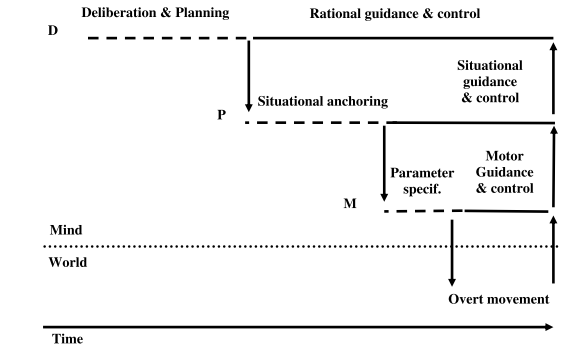
\includegraphics[width=0.8\textwidth]{figs/Chapter1/Pacherie.png}
    \caption{The intentional cascade by Pacherie. Distal, Proximal and Motor intentions coexist at the same time, each one controlling the action at a different level.}
    \label{fig:Pacherie}
\end{figure}

In \cite{pacherie2011phenomenology}, Pacherie extends these three levels to Joint Action. In the same way as before, these three new levels coexist at the same time, each one controlling the Joint Action at a different level.

\paragraph{Shared Distal Intention:}
Where \textit{Distal Intention} was responsible for intention, \textit{Shared Distal Intention} is responsible for joint intention. When performing a Joint Action, this level is the one responsible for the shared goal and the Shared Plan. As said in Sec.~\ref{subsec:commitment}, the agent does not have a whole representation of the Shared Plan here and part of his representation will be executed by someone else.

\paragraph{Shared Proximal Intention:}
This level has the same responsibilities as \textit{Proximal Intention}, however, the anchoring of the action plan needs to take care of the Joint Action partners and to be done in a coordinated way. During the monitoring part, the choices made previously need to be adapted to the others behavior.

\paragraph{Coupled Motor Intention:}
As for \textit{Motor Intention}, this level is responsible for the motor commands of the agent. During Joint Action, this level will be the one responsible for precise spatio-temporal coordination for the actions which need it (e.g. holding an object together).


\subsection{A three levels robotics architecture}

\label{subsec:Archi}

Ten years before Pacherie came with her action theory with three levels, the field of autonomous robotics was trying to build architectures and was already intuitively designing three similar levels. A first implemented architecture for autonomous robots is presented in \cite{alami1998architecture}, organized around these three levels (fig.~\ref{fig:FirstArchi}).

\begin{figure}[!h]
	\centering
    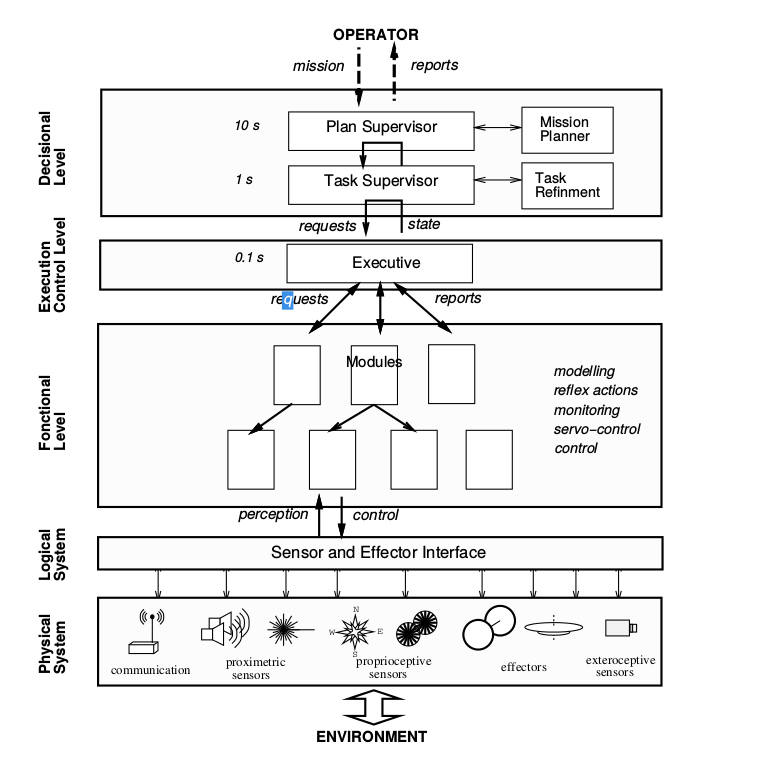
\includegraphics[width=0.8\textwidth]{figs/Chapter1/ArchitectureHold.png}
    \caption{One of the first architectures for autonomous robots. The architecture is divided in three main parts: decision, execution and functional levels.}
    \label{fig:FirstArchi}
\end{figure}

\paragraph{Decision level:}
This level can be compared to the \textit{Distal Intention} level of Pacherie. It is the one responsible for producing a task plan and supervising it. It sends actions to execute and receives reports from the \textit{execution level}.

\paragraph{Execution level:}
This level can be compared to the \textit{Proximal Intention} level of Pacherie. It receives from the \textit{decision level} the sequence of actions to be executed and selects, parametrizes and synchronizes dynamically the adequate functions of the \textit{functional level}.

\paragraph{Functional level:}
This level can be compared to the \textit{Motor Intention} level of Pacherie. It includes all the basic robot action and perception capacities (motion planning, vision, localization, tracking motion control...). 

\bigskip
In the past years, this architecture has been developed and adapted to the field of HRI. In recent works, we presented in \cite{devin2016some} a theoretical version of the architecture adapted to human-robot Joint Action and still based on the three levels of Pacherie (fig.~\ref{fig:ArchiThreeLevels}). The implemented version of this architecture will be presented in Chapter~\ref{ch:Sup}, where my contribution in the architecture will also be highlighted.

\begin{figure}[!h]
	\centering
    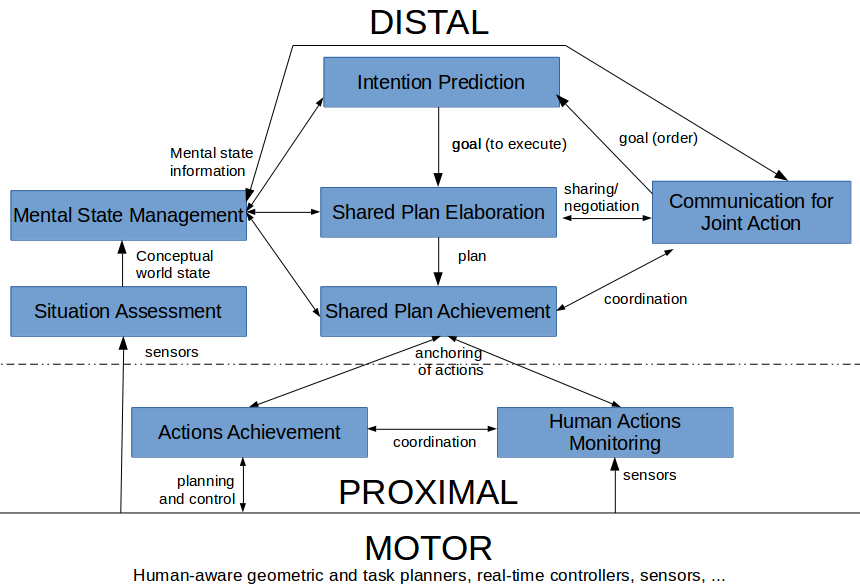
\includegraphics[width=\textwidth]{figs/Chapter1/architecture.png}
    \caption{Recent architecture for human-robot Joint Action. The architecture is organized in three levels corresponding to the ones defined by Pacherie.}
    \label{fig:ArchiThreeLevels}
\end{figure}

\paragraph{Distal level:}
As for \textit{Shared Distal Intention}, this level is responsible for goals and Shared Plans management. At this level, the robot is supposed to reason on its environment with high level representations. To do so, the robot is equipped with a \textbf{Situation Assessment} module which builds a symbolic representation of the robot environment. To be able to also reason about the humans knowledge, the robot is equipped with a \textbf{Mental State Management} module which constantly estimates humans mental states. With this information, the \textbf{Intention prediction} module is able to estimate humans intention and if the robot should propose its help or not. This module determines the goal of the robot and allows, during its execution, to monitor other agents engagement. Once the goal chosen, the \textbf{Shared Plan Elaboration} module allows the robot to construct and negotiate a Shared Plan to achieve the goal. Then, the \textbf{Shared Plan Achievement} module monitors the good execution of this Shared Plan. The last part of this level is the \textbf{Communication for Joint Action} module which allows the robot to verbally and non-verbally communicate during Joint Action. 

\paragraph{Proximal level:}
As for \textit{Shared Proximal Intention}, this level is in charge of anchoring the Shared Plan actions in the current situation. This level is composed of two parts: the \textbf{Actions Achievement} module which allows to call the adequate motor modules at the right time in order to perform robot actions and the \textbf{Human Actions Monitoring} module which allows to recognize and interpret humans actions with regard to the Shared Plan. These two modules communicate in order to coordinate robot actions to the humans ones.

\paragraph{Motor level:}
As for \textit{Coupled Motor Intention}, this level is in charge of motor commands of the robot. This level includes all modules allowing to control the robot actuators and interprets data from sensors. These modules, or at least a part of them, also take into account the humans as, for example, the human-aware geometric task and motion planner.

\ifdefined\included
\else
\bibliographystyle{StyleThese}
\bibliography{These}
\end{document}
\fi
